\documentclass{scrartcl}
\usepackage{amssymb}
\usepackage{amsmath}
\usepackage{tikz}
\usetikzlibrary{knots,hobby,decorations.pathreplacing,shapes.geometric,calc}

\def\centerarc[#1](#2)(#3:#4:#5)% Syntax: [draw options] (center) (initial angle:final angle:radius)
{ \draw[#1] ($(#2)+({#5*cos(#3)},{#5*sin(#3)})$) arc (#3:#4:#5); }

\begin{document}
	
%	\begin{tikzpicture}		%plain Venn diagram
	%Real
%	\draw[very thick] (0,0) circle (1.5cm);
%	\node at (-1.25,-1.75) {R\'{e}el};
	%
	%Symbolic
%	\draw[very thick] (1,1.5) circle (1.5cm);	
%	\node at (3.25,-1.75) {Symbolique};
	%
	%Imaginary
%	\draw[very thick] (2,0) circle (1.5cm);
%	\node at (1,3.35) {Imaginaire};
	%
	%other labels
%	\node at (1,0.45) {a};
%	\node at (0.2,0.9) {JA};
%	\node at (1,-0.4) {J$\Phi$};
%	\node at (1.8,0.9) {Sens};
%	\node at (1,2.1) {Corps};
%	\end{tikzpicture}
	
%	\vspace{1cm}
	
	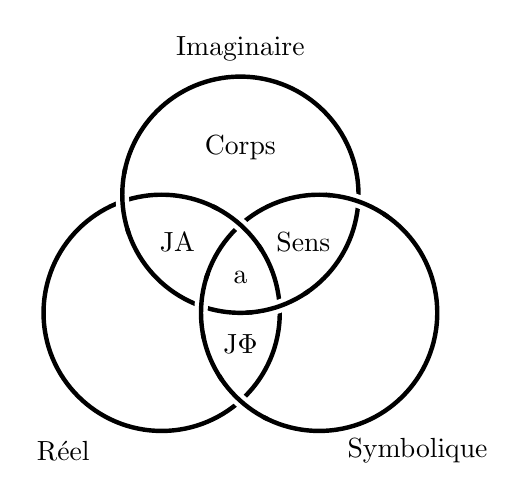
\begin{tikzpicture}		%NB: need the knots package for this
	\begin{knot}[
	%  draft mode=crossings,
	flip crossing=3				%note: crossings change if this number is set to 1 or 2
	]							%note: order of the circles matters -- needs to be ISR
	\strand[black, ultra thick] (2,0) circle[radius=1.5cm];		%Imaginary
	\strand[black, ultra thick] (1,1.5) circle[radius=1.5cm];	%Symbolic
	\strand[black, ultra thick] (0,0) circle[radius=1.5cm];		%Real
	\end{knot}
	
	\node at (1,3.35) {Imaginaire};
	\node at (3.25,-1.75) {Symbolique};
	\node at (-1.25,-1.75) {R\'{e}el};
	
	%other labels
	\node at (1,0.45) {a};
	\node at (0.2,0.9) {JA};
	\node at (1,-0.4) {J$\Phi$};
	\node at (1.8,0.9) {Sens};
	\node at (1,2.1) {Corps};
	\end{tikzpicture}

	\vspace{2.5cm}
	
	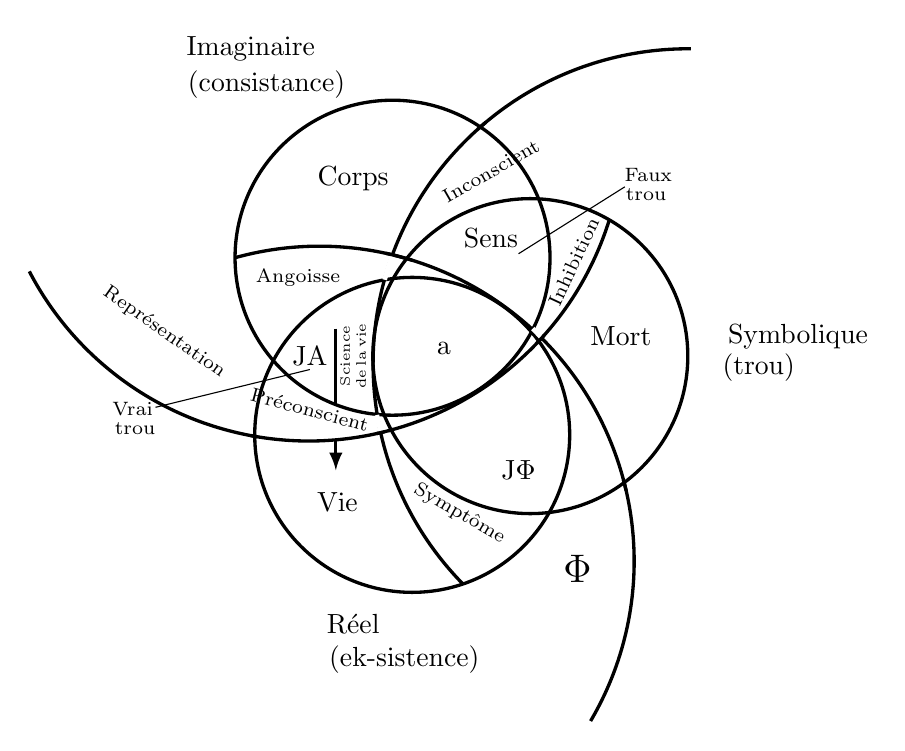
\begin{tikzpicture}		%fancy Venn diagram
	%Real
	\draw[very thick] (0,0) circle (2cm);
	\node at (-0.75,-2.4) {R\'{e}el};
	\node at (-0.1,-2.85) {(ek-sistence)};
	
	%Symbolic
	\draw[very thick] (1.5,1) circle (2cm);	
	\node at (4.9,1.25) {Symbolique};
	\node at (4.4,0.85) {(trou)};
	
	%Imaginary
	\draw[very thick] (-0.25,2.25) circle (2cm);
	\node at (-2.05,4.9) {Imaginaire};
	\node at (-1.85,4.45) {(consistance)};
	
	%other labels
	\node at (0.4,1.1) {a};
	\node at (-0.95,-0.85) {Vie};
	\node at (-1.3,1) {JA};
	\node at (-1.45,2) {{\scriptsize Angoisse}};
	\node at (2.65,1.25) {Mort};
	\node at (3,3.3) {{\scriptsize Faux}};
	\node at (2.97,3.05) {{\scriptsize trou}};		\draw (2.7,3.15)--(1.35,2.3);
	\node at (1.35,-0.45) {J$\Phi$};
	\node at (2.1,-1.7) {{\Large $\Phi$}};
	\node at (1,2.5) {Sens};
	\node at (-0.75,3.25) {Corps};
	\node at (-0.85,1) {\rotatebox{90}{{\tiny Science}}};
	\node at (-0.65,1) {\rotatebox{90}{{\tiny de$\,$la$\,$vie}}};
	\draw [very thick]	(-0.97,1.35)--(-0.97,0.38);						%'arrow' shaft
	\draw [->, >=latex, very thick]	(-0.97,-0.05)--(-0.97,-0.45);		%arrowhead
	\node at (0.6,-1) {\rotatebox{330}{{\scriptsize Sympt\^{o}me}}};
	\node at (2.05,2.2) {\rotatebox{65}{{\scriptsize Inhibition}}};
	\node at (-3.15,1.3) {\rotatebox{325}{{\scriptsize Repr\'{e}sentation}}};
	%\node at (-3.35,0.2) {{\scriptsize Vrai}};
	%\node at (-3.32,-0.05) {{\scriptsize trou}};	\draw (-3.1,0.2)--(-1.25,0.8);
	\node at (-3.55,0.33) {{\scriptsize Vrai}};
	\node at (-3.52,0.08) {{\scriptsize trou}};
	
	
	%beginning of arc	%NB: these aren't exactly correct
	%\node at (2.5,2.72) {\textcolor{red}{.}};		%horizontal arc	cf. Sens
	%\node at (0.65,-1.9) {\textcolor{red}{.}};		%vertical arc	cf. Reel
	%\node at (-2.25,2.25) {\textcolor{red}{.}};	%diagonal arc	cf. Angoisse	
	%end of arc
	%\node at (-4.75,2) {\textcolor{red}{.}};		%horizontal arc	cf. Angoisse
	%\node at (4,4.75) {\textcolor{red}{.}};		%vertical arc	cf. Imaginaire / Faux
	%\node at (2.25,-3.5) {\textcolor{red}{.}};		%diagonal arc	cf. Reel / Mort
	
	%arcs
	\draw[black, very thick]   (2.5,2.72) arc (342.5:207.5:4cm);	%horizontal
	\draw[black, very thick]  (-2.25,2.25) arc (105.5:-30.5:4cm);	%diagonal, finished
	\draw[black, very thick] (0.65,-1.9) arc (224.5:89.5:4cm);		%vertical, finished
	
	%erasing part of circles
	\centerarc[white,line width=1.8](0,0)(180.5:152:2)		%covers Real circle, near "preconscient"
	\centerarc[white,line width=1.8](1.5,1)(277:306.5:2)	%covers Symb circle, near \Phi
	\centerarc[white,line width=1.8](-0.25,2.25)(22:56:2)	%covers Imag circle, near "inconscient"
	
	\node at (1,3.35) {\rotatebox{30}{{\scriptsize Inconscient}}};
	\node at (-1.3,0.32) {\rotatebox{345}{{\scriptsize Pr\'{e}conscient}}};
	\draw (-3.26,0.35)--(-1.3,0.83);	%line from Vrai to JA
	
	\centerarc[white,line width=1.7](1.5,1)(142:150.5:2)		%covers Symb circle, upper
	\centerarc[white,line width=1.7](1.5,1)(202:208:2)			%covers Symb circle, lower
	\centerarc[white,line width=1.7](0,0)(37:40.5:2)			%covers Real circle
	
	%erasing part of arcs
	%\node at (-0.4,0.05) {\textcolor{red}{.}};
	\draw[white, line width=1.7]  (-0.4,0.049) arc (195:192:4cm);
	%\node at (-0.35,1.97) {\textcolor{red}{.}};
	\draw[white, line width=1.7]  (-0.35,1.97) arc (165:160.5:4cm);
	%\node at (1.55,1.33) {\textcolor{red}{.}};
	\draw[white, line width=1.7]  (1.53,1.35) arc (45.3:43:4cm);
	
	%re-doing parts of circles that were erased
	\centerarc[black,very thick](0,0)(328:333:2)
	\centerarc[black,very thick](0,0.0004)(95:103:2)
	\centerarc[black,very thick](1.5,1)(85:89:2)
	\centerarc[black,very thick](-0.25,2.25)(260:270:2)
	\centerarc[black,very thick](-0.2496,2.25)(330:335:2)
	\centerarc[black,very thick](-0.25,2.25)(219:222:2)
	
	%re-doing parts of arcs that were erased
		%SE: find center for a given arc, then use \centerarc
	%vertical arc: 1 fix
	%\node at (0.83,3.88) {\textcolor{red}{.}};		%vertical arc
	\draw[black, very thick]  (0.831,3.88) arc (131.9:129.9:4cm);
	%
	%diagonal arc: 2 fixes
	%\node at (2.69,-0.58) {\textcolor{red}{.}};	%diagonal arc, near \Phi
	\draw[black, very thick]  (2.6825,-0.57) arc (15:13:4cm);
	%\node at (0,2.21) {\textcolor{red}{.}};
	\draw[black, very thick]  (0,2.2175) arc (72.75:77.75:4cm);
	%
	%horizontal arc: 3 fixes
	%\node at (-2.05,-0.015) {\textcolor{red}{.}};
	\draw[black, very thick]  (-2.05,-0.0093) arc (259.3:260.5:4cm);
	%\node at (-0.3,0.06) {\textcolor{red}{.}};
	\draw[black, very thick]  (-0.305,0.052) arc (284.5:285.5:4cm);
	\draw[black, very thick]  (-0.45,0.0168) arc (282.6:284.1:4cm);
	%\node at (1.58,1.15) {\textcolor{red}{.}};
	\draw[black, very thick]  (1.581,1.1622) arc (316.3:318.3:4cm);
	
	\end{tikzpicture}
	
\end{document}